\chapter{Diseño e Implementación} \label{chap:analisisExperimentación}


\section{Diseño Pedagógico}

El diseño pedagógico se centra en el aprendizaje basado en problemas \cite{de2008aprendizaje}. Concretamente, se introduce la teoría relevante, que puede incluir explicaciones de texto, imágenes ilustrativas, y en ocasiones, material en formato de video. Una vez que el usuario ha absorbido el contenido teórico, se le presentan problemas prácticos relacionados para resolver.

Existen dos categorías principales de ejercicios, cada una con un peso distinto en la estructura de aprendizaje:

\begin {enumerate}
\item Ejercicios estándar: Son problemas prácticos que refuerzan la comprensión del usuario sobre el tema.

\item Ejercicios clave (\textit{key\_exercise}): Estos ejercicios desempeñan un papel crucial en la progresión del usuario. Son indicativos de si el usuario ha comprendido los requisitos fundamentales del tema en cuestión. Se deben completar estos ejercicios para avanzar al siguiente tema o módulo. Si el usuario no logra superar estos ejercicios en un primer intento, se le presentan ejercicios adicionales para reforzar su comprensión antes de volver a intentarlo.
\end{enumerate}

La plataforma corrige automáticamente para los módulos de C++, Java y Python, tal como se mencionó con anterioridad. Sin embargo, para el módulo de HTML+CSS+JS, se requiere una revisión manual por parte de un instructor. Esta revisión no solo califica el ejercicio, sino que también proporciona comentarios constructivos para guiar al usuario hacia la solución correcta.

Además de la corrección, la plataforma evalúa la limpieza y estructura del código presentado, ya que es esencial para un buen aprendizaje. Por lo tanto, se proporciona una retroalimentación detallada al estudiante no solo sobre la corrección de su respuesta, sino también sobre cómo mejorar y optimizar su código.

Finalmente, la plataforma tiene la capacidad de compilar ejercicios, permitiendo la verificación y corrección del código antes de su envío.

\section{Arquitectura del Sistema}

La interacción del usuario en el Frontend se lleva a cabo utilizando tecnologías estándar como HTML sin emplear \textit{frameworks} adicionales para su desarrollo. Además, la interfaz es \textit{Web Responsive}, lo que garantiza su adaptación a variados dispositivos. Desde el punto de vista de la seguridad, se han implementado medidas como la validación de entradas, previniendo así amenazas como los ataques XSS. Los datos de sesión se conservan en el cliente mediante cookies.

Por otro lado, el Backend se ha desarrollado con Flask. Se encarga de administrar las API RESTful y de establecer una conexión ininterrumpida con la base de datos PostgreSQL. La biblioteca \textit{flask\_login} respalda las funcionalidades de autenticación y autorización, aportando una capa de seguridad adicional. La lógica de negocio del sistema reside principalmente en el Sistema de Tutoría Inteligente (ITS). Este subsistema es el encargado de la elección y evaluación de ejercicios, ofreciendo retroalimentación y monitoreando el avance del estudiante.

En relación con la seguridad del Backend, se han establecido roles y restricciones de acceso coherentes con las reglas de negocio previamente determinadas. Aunque la arquitectura actual no posee herramientas concretas orientadas a la escalabilidad, está concebida para ser resistente y estable.

Es esencial destacar que, la estructura general del sistema sigue el patrón Modelo-Vista-Controlador (MVC). La Vista reside en el Frontend, y el Controlador y Modelo en el Backend \ref{fig:arqsistema}. Este patrón facilita la distinción entre la lógica de la interfaz de usuario y las operaciones, simplificando su mantenimiento.

\begin{figure}[H]
    \centering
    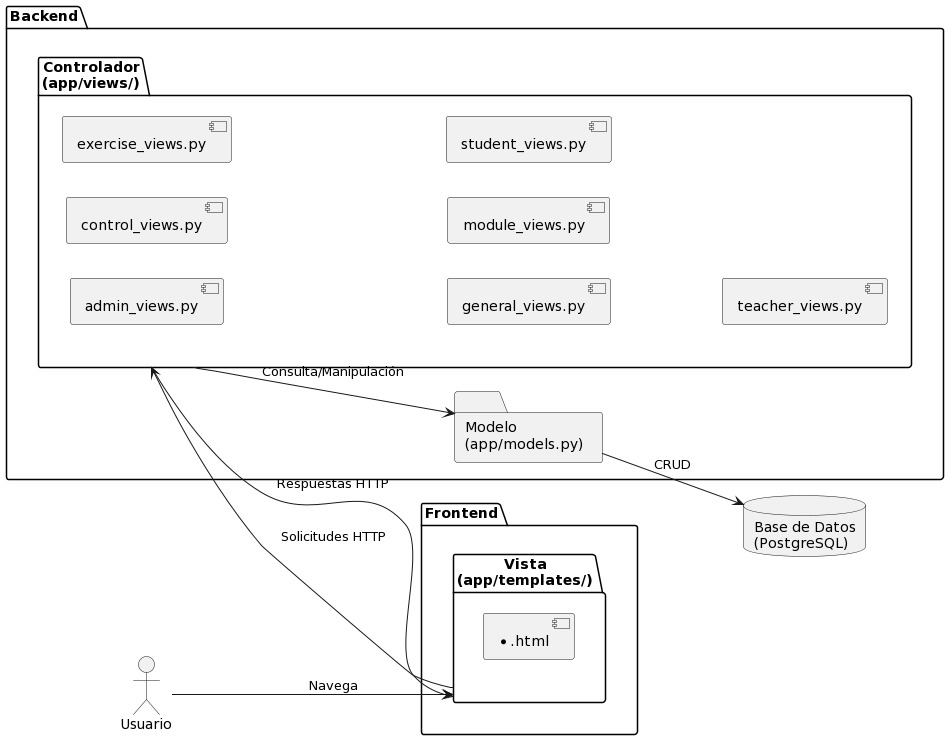
\includegraphics[width=0.55\textwidth]{imagenes/ArquitecturaDeSistema.jpeg}
    
    \caption{Arquitectura de sistema}
    \label{fig:arqsistema}
\end{figure}

\section{Diseño de Base de Datos}

La arquitectura de nuestra base de datos es el resultado de un exhaustivo análisis y diseño. Su estructura no solo atiende a las necesidades actuales, sino que también se anticipa a los retos futuros. A continuación, detallamos algunos de los elementos clave y las consideraciones adoptadas en su construcción:

\begin{enumerate}
    \item \textbf{Tablas principales y su significado}: Las tablas como \textit{users}, \textit{modules}, \textit{exercises}, \textit{questions} y \textit{theory} son la columna vertebral de la base de datos. En ellas, se almacena la información medular que alimenta las funcionalidades centrales del sistema. Estas tablas, además de contener datos primordiales, están interconectadas a través de relaciones específicas. Garantizando, así, la coherencia y la integridad de la información en todo momento.
    
    \item  \textbf{La importancia de los índices}: Los índices son herramientas fundamentales para acelerar las consultas y garantizar un rendimiento óptimo. Dentro de la base de datos, su uso es estratégico. Existen índices únicos, como el \textit{users\_email\_key}, que aseguran la singularidad de ciertos registros. Por ejemplo, en el caso del correo electrónico, se garantiza que no existan duplicados. Los índices compuestos, como \textit{student\_modules\_student\_id\_module\_id\_key}, son esenciales para optimizar las consultas que abarcan múltiples campos. Las tablas intermedias, que representan relaciones entre otras, también hacen uso de índices. En este caso, \textit{exerciserequirements} y \textit{theoryrequirements}. Estos índices, principalmente compuestos, agilizan y refuerzan las consultas relacionales.

    \item \textbf{La normalización como estándar}: Uno de los principios fundamentales que se ha seguido es la normalización. Al estructurar la información de esta manera, se minimiza la redundancia y maximiza la eficiencia.

    \item \textbf{Relaciones bien definidas}: La claridad en las relaciones entre tablas es esencial. Gracias a las claves primarias y foráneas, se ha conseguido una red de relaciones que no solo facilita la integración y consulta de datos sino que también refuerza la integridad de los mismos.

    \item \textbf{Mirando hacia el futuro}: Más allá de las necesidades actuales, el diseño busca ser resiliente y adaptable. Pretendiendo que cualquier adición futura, ya sea en funcionalidades o módulos, se integre sin grandes complicaciones.
\end {enumerate}


En resumen, la base de datos del sistema es robusta, detallada y diseñada para crecer. Teniendo como aspiración que, más allá de ser un simple almacén de datos, sea una herramienta eficiente que potencie la experiencia del usuario y facilite el trabajo de la ITS.

\newpage

\begin{figure}[H]
    \centering
    \begin{sideways}
        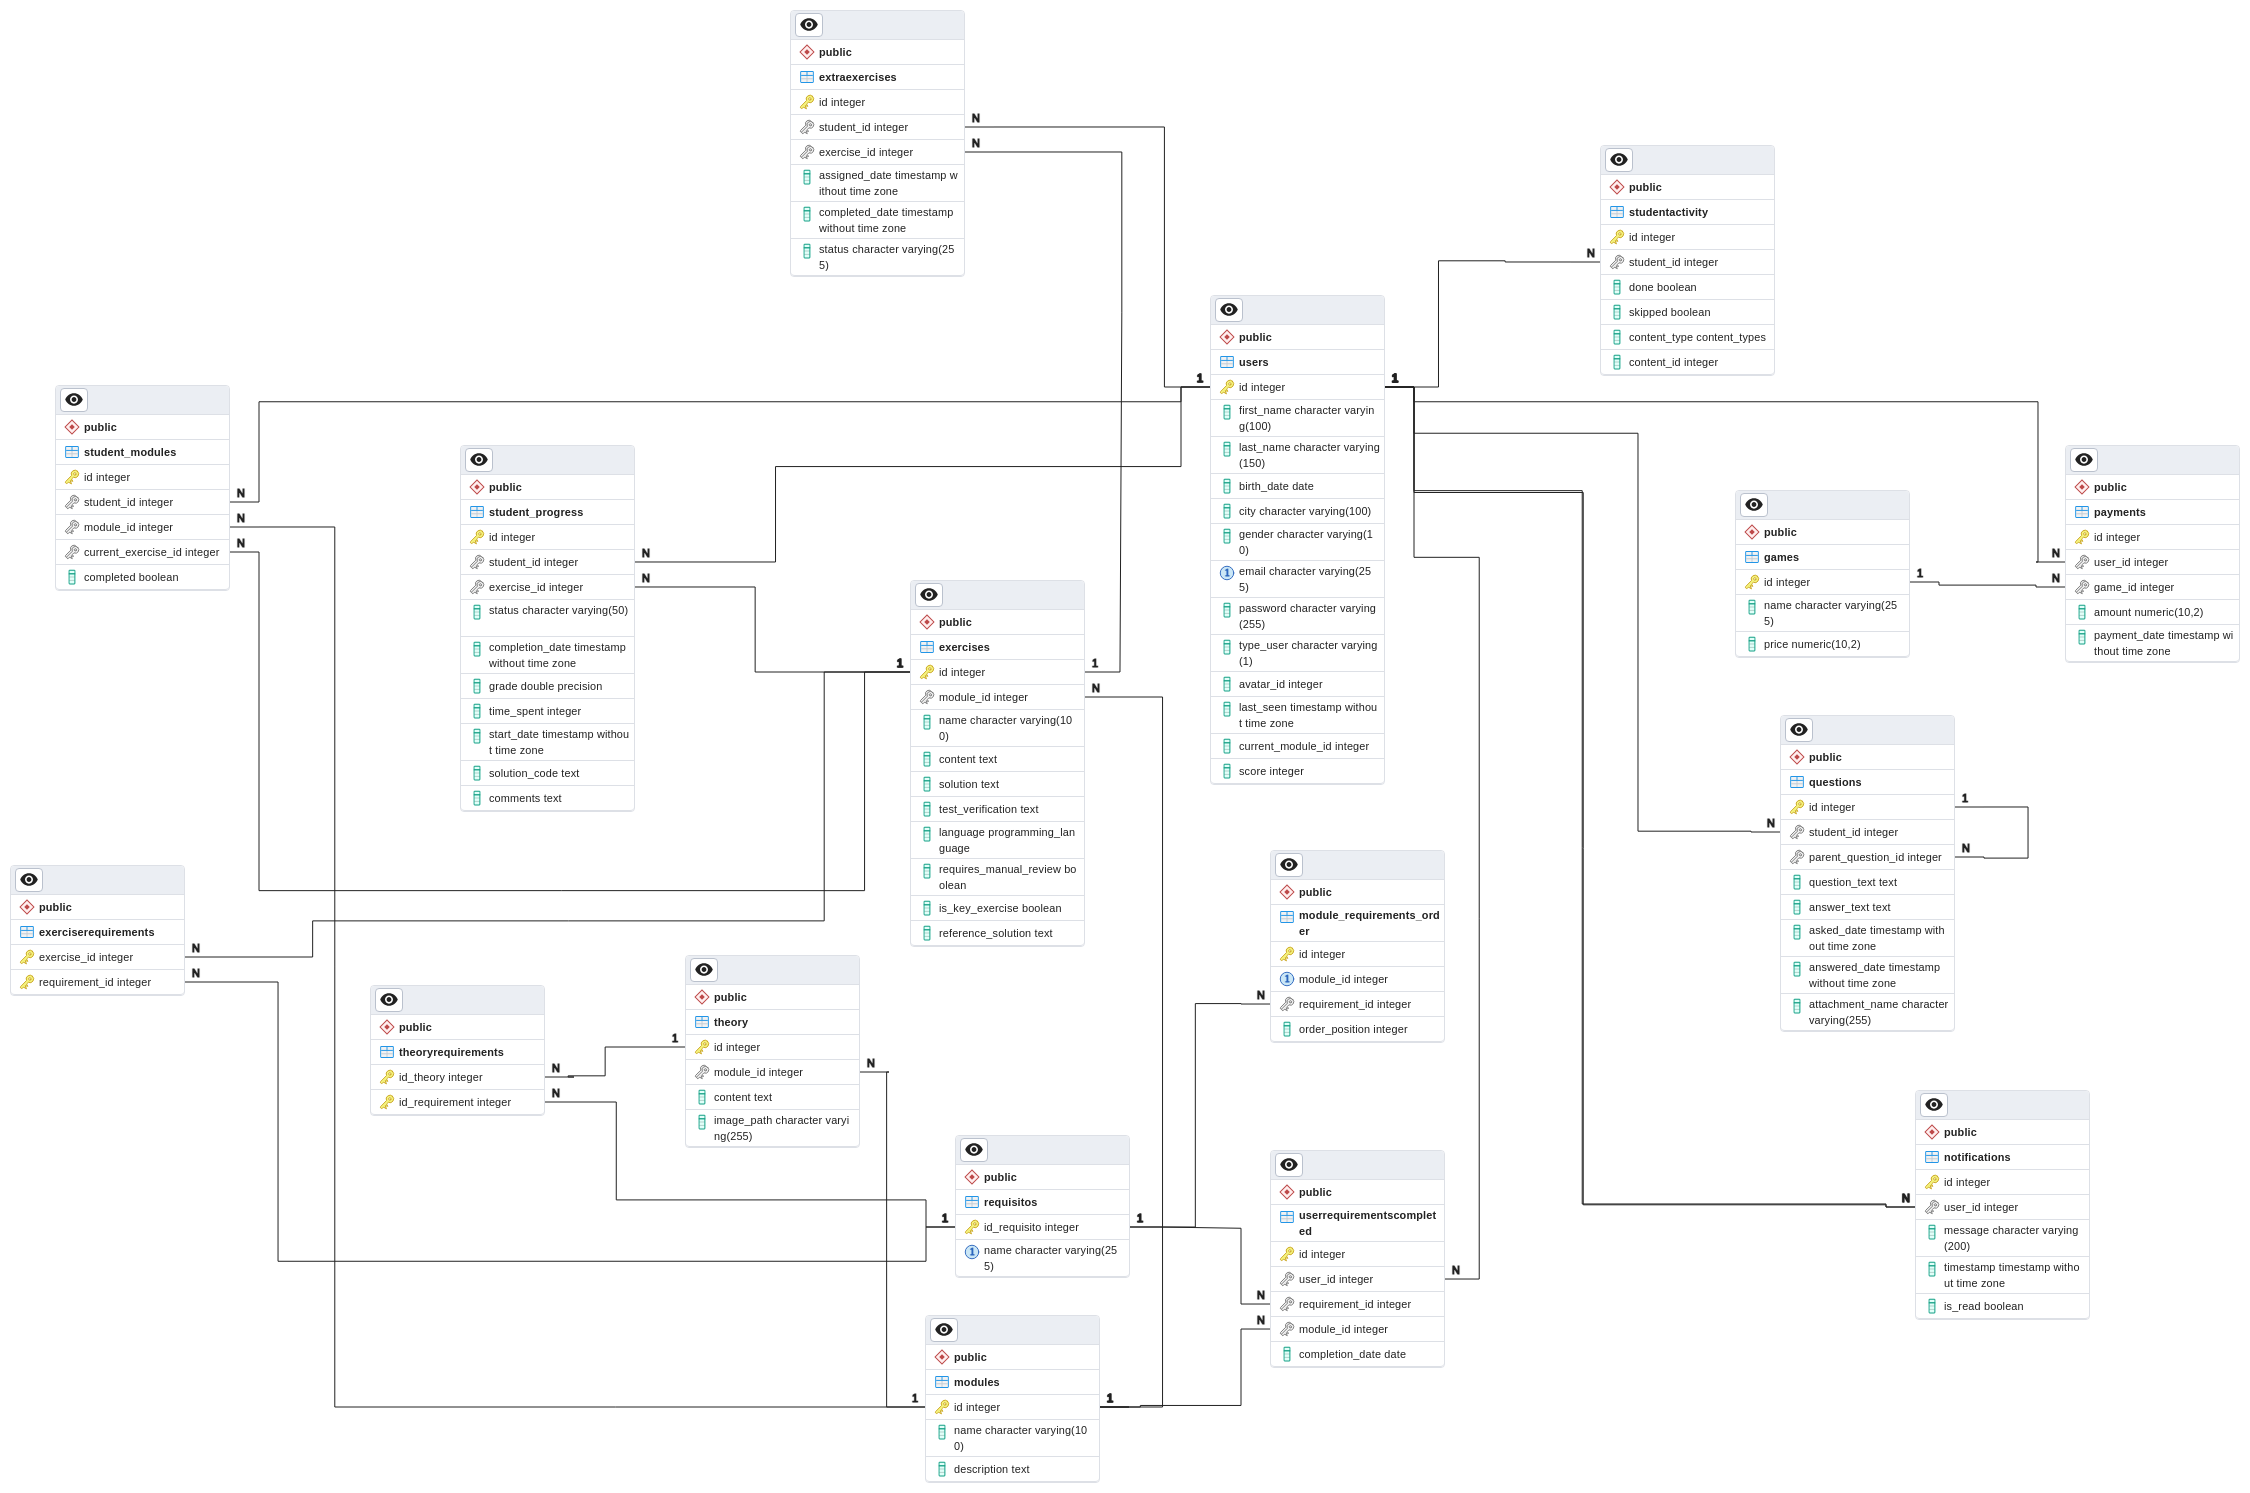
\includegraphics[width=1.8\textwidth]{imagenes/er.png}
    \end{sideways}
    \caption{Diagrama del modelo de datos}
    \label{fig:modeladodedatos}
\end{figure}

\section{Interfaces de Usuario}
\subsection{Mockups o Capturas de Pantalla}
\subsection{Interacción Usuario-Sistema}
Detalles de la interacción del usuario con el sistema.

\section{Implementación de Algoritmos}
\subsection{Algoritmo para la corrección y Evaluación de calidad del código}

El verdadero reto comienza tras la entrega de un ejercicio por parte del estudiante. La lógica de corrección evalúa el código en términos de precisión y calidad. Si un código no alcanza un estándar mínimo, el sistema propone ejercicios adicionales, reforzando así las áreas de mejora del estudiante \ref{fig:correccion}. La justificación detrás de esta lógica se centra en la premisa de que la repetición y el refuerzo son esenciales para consolidar el aprendizaje. Además, al establecer estándares de calidad, se fomentan las buenas prácticas de programación desde las etapas iniciales de formación.

\begin{figure}[H]
    \centering
    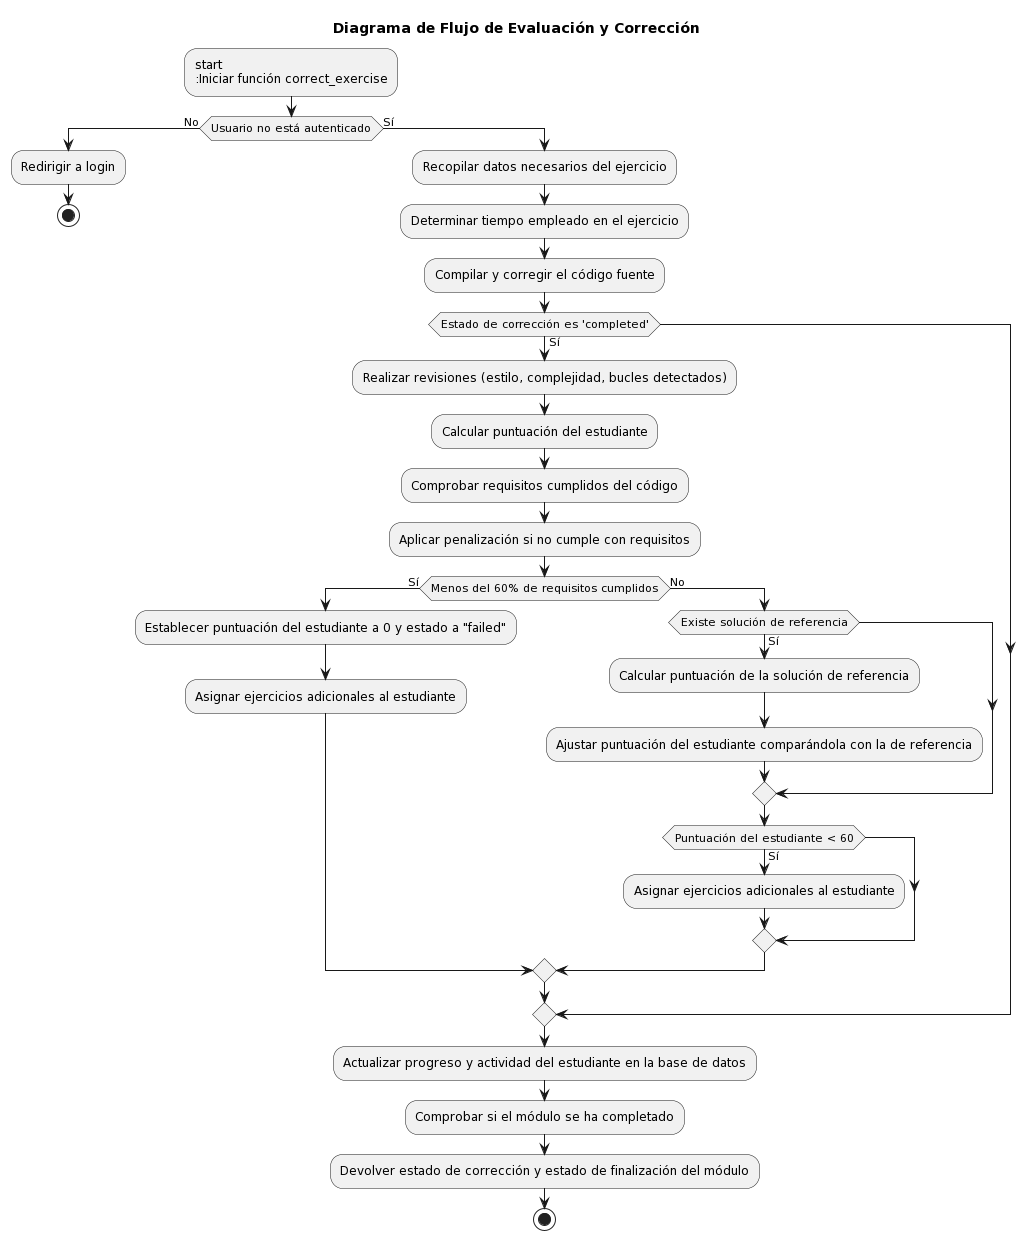
\includegraphics[width=\textwidth]{imagenes/correcionejercicios.png}
    \caption{Diagrama de flujo para la selección de ejercicios}
    \label{fig:correccion}
    \end{figure}

\subsection{Algoritmo para la selección y evaluación de ejercicios}

El sistema prioriza la progresión estructurada del estudiante. Al ingresar, la plataforma identifica ejercicios en curso o determina el próximo paso en función de los requisitos del módulo. Esta estructura garantiza que, antes de enfrentarse a cualquier tarea, los conceptos teóricos relevantes sean presentados al estudiante \ref{fig:seleccion}. Esta estrategia se fundamenta en la pedagogía moderna, que sugiere que la teoría y la práctica deben ir de la mano para un aprendizaje óptimo.

\begin{figure}[H]
\centering
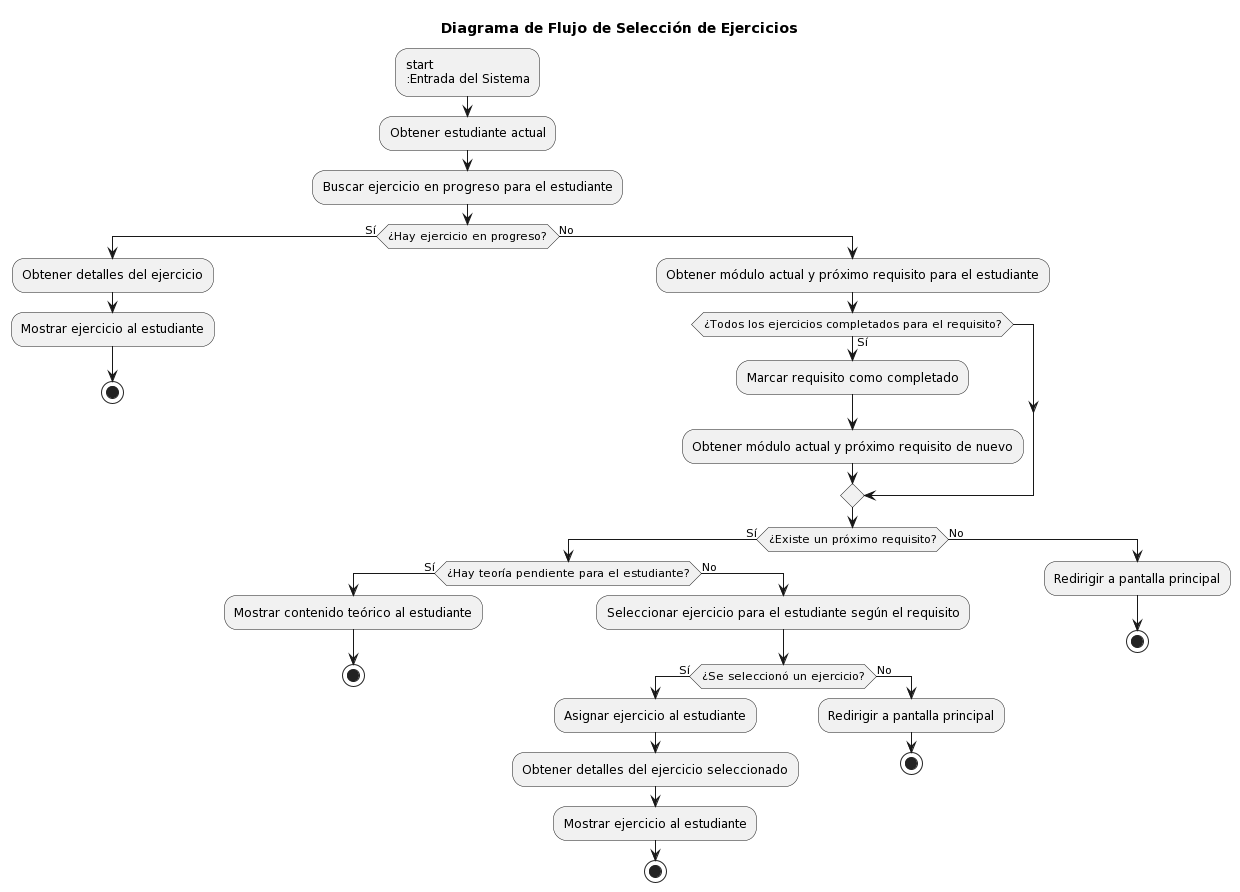
\includegraphics[width=\textwidth]{imagenes/seleccionejercicios.png}
\caption{Diagrama de flujo para la selección de ejercicios}
\label{fig:seleccion}
\end{figure}

\section{Tecnologías y Herramientas}
Enumere las tecnologías, lenguajes de programación, frameworks y bibliotecas utilizadas.

\section{Implementación de Módulos de Aprendizaje Adaptativo}
Describa cómo el sistema se adapta al progreso del estudiante.
